% !TEX encoding = UTF-8
% !TEX TS-program = pdflatex
% !TEX root = ../tesi.tex

%**************************************************************
\chapter{Background}
\label{cap:descrizione-stage}
%**************************************************************

\intro{This section briefly covers, in section \ref{sec:ogp}, the online gaming panorama, in section \ref{sec:csgo} explores the game (CS:GO), and in section \ref{sec:ml} describes the machine learning techniques involved.}\\

%**************************************************************
\section{\label{sec:ogp}Online gaming panorama}

	There are more than 3.2 billion players on Earth\cite{site:statista}. 
	Many people play to have some form of entertainment. 
	There are numerous games, and a large portion of them has some form of online interaction. 
	For the work described, we chose among the most popular online video games in 2021. 
	Table \ref{tab:Game players table} lists some of the candidates. 	
	
	\begin{table}[!h]
	
		\centering
		
		\caption{\label{tab:Game players table}Video game table. The monthly players take in consideration July 2021}
		
		\begin{tabular}{|c|c|c|c|c|c|c|}
			
			\hline
			 & \makecell{\textbf{{\footnotesize Monthly}} \\ \textbf{{\footnotesize Players}}} & \makecell{\textbf{{\footnotesize Release}} \\ \textbf{{\footnotesize Year}}} & \makecell{\textbf{{\footnotesize Free}} \\ \textbf{{\footnotesize To Play}}} & 
			 \makecell{\textbf{{\footnotesize Tracking}} \\ \textbf{{\footnotesize Websites}}} & \makecell{\textbf{{\footnotesize Replay}} \\ \textbf{{\footnotesize availability}}} & \makecell{\textbf{{\footnotesize Parser}} \\ \textbf{\footnotesize availability}}} \\			
			\hline
			\textbf{{\footnotesize Minecraft}} & {\footnotesize 162,055,144} & {\footnotesize 2011} & {\footnotesize No} & {\footnotesize Yes} & {\footnotesize Low} & {\footnotesize Low} \\
			\hline
			\textbf{{\footnotesize LOL}} & {\footnotesize 128,014,473} & {\footnotesize 2009} & {\footnotesize Yes} & {\footnotesize Yes} & {\footnotesize Medium} & {\footnotesize Low}\\
			\hline
			\textbf{{\footnotesize Fortnite}} & {\footnotesize 283,665,016} & {\footnotesize 2017} & {\footnotesize Yes} & {\footnotesize Yes} & {\footnotesize High} & {\footnotesize Medium}\\
			\hline
			\textbf{{\footnotesize PUBG}} & {\footnotesize 530,844,730} & {\footnotesize 2016} & {\footnotesize No} & {\footnotesize Yes} & {\footnotesize Medium} & {\footnotesize High}\\
			\hline
			\textbf{{\footnotesize DOTA 2}} & {\footnotesize 460,661} & {\footnotesize 2013} & {\footnotesize Yes} & {\footnotesize Yes} & {\footnotesize High} & {\footnotesize High}\\
			\hline
			\rowcolor{Gray}
			\textbf{{\footnotesize CS:GO}} & {\footnotesize 36,011,477} & {\footnotesize 2012} & {\footnotesize Yes} & {\footnotesize Yes} & {\footnotesize High} & {\footnotesize High}\\
			\hline

		\end{tabular}
	
	\end{table}
	Source: activeplayer.io\cite{site:activePlayerLOL}\cite{site:activePlayerFortnite}\cite{site:activePlayerPUBG}\cite{site:activePlayerMinecraft}\cite{site:activePlayersDota}\cite{site:activePlayersCSGO}
	
	\noindent Although these are all possible candidates, DOTA 2 was, of course, not eligible because it was the subject of the previous work. 
	Out of all the other possibilities, we decided to work on CS:GO for the difference with DOTA 2, the replay availability, and the parser availability.  

%**************************************************************	
	
\section{\label{sec:csgo}The game and its mechanics}

	Counter-Strike: Global Offensive is a multiplayer, objective-based, \gls{FPS} released by Valve in 2012 and available for free on \gls{Steam}. 
	It is the fourth chapter of the Counter-Strike series.\\
	The player controls a character that can move around on the map and must complete the given objective. 
	There are eight different game modes, but the one considered for this work is the competitive mode. 
	The competitive mode is a best-of-30 match. 
	The first team to score 16 wins is the winner of the whole competition. 
	It is still possible to tie if the score is 15-15. 
	A rating system helps to match together players with similar skills. 
	
	In competitive mode, there are two main modes: 
	
	\begin{itemize}
	
		\item \textbf{Bomb scenery}: The terrorists must place an explosive in one of the two sites (identified as A or B, as shown in Figure \ref{fig:map}) and make sure it explodes within a time limit. 
		The counter-terrorists must prevent the bomb from exploding. There are two ways to do so: stop the planting of the bomb or defuse it.
		
		\item \textbf{Hostage scenery}: In the map some hostages must be escorted to an extraction point by the counter-terrorists. The terrorist's objective is, on the other side, prevent the hostages to escape. 
		Killing them is forbidden.
	
	\end{itemize}
	
	\begin{figure}[!h] 
		\centering 
		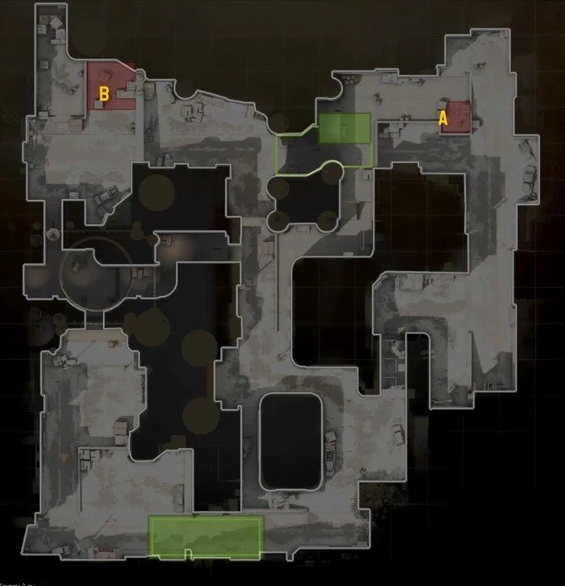
\includegraphics[scale=0.6]{game/map.png}
		\caption{\label{fig:map}Example of Dust2, a CS:GO map}
	\end{figure}
	
	Both these modes need two opposed teams: terrorists and counter-terrorists (shown in Figure \ref{fig:teams}). 
	These teams have some objectives to achieve. 
	During every round, every player earns in-game currency based on single actions (such as kills) or team actions (for example clearing objectives). 
	At the same time, negative actions (such as killing a teammate) leads to losing the in-game money. 
	Every player can use the currency earned in the previous round to buy weapons or other utilities for the current round. 
	
	\begin{figure}[!h] 
		\centering 
		
\includegraphics[width=0.9\columnwidth]{game/csgo_teams.png}
		\caption{\label{fig:teams}CS:GO teams: counter-terrorists and terrorists}
	\end{figure}

	In CS:GO, there are nine different maps for competitive play, of which Dust2 (in Figure \ref{fig:map}) is an example. 
	Every map has some predefined spawn points for both terrorists and counter-terrorists. 
	There are also two predefined areas to plant the bomb (labeled as A and B, as previously mentioned) and a predefined extraction point for the hostage scenery.

	\paragraph{\textsc{The match}}\\

		A competitive match is composed of 30 rounds. Every round is divided into two parts:
		
		\begin{itemize}
		
			\item \textbf{The item purchase}:\\
				At the beginning of the match, there is some time dedicated to purchasing, from the in-game store (Figure \ref{fig:store}) the equipment necessary for the round. 
				The purchasing can include better or different weapons or other utilities to win.
			
			\item \textbf{The match}:\\
				The match itself is, of course,  the core part of the game. In this phase, the players try to achieve their objectives. 
				For the terrorists' team, the goal is to plant the bomb and make it explode or prevent the hostages from escaping. 
				On the other side, the counter-terrorists must prevent the bomb from exploding or make the hostages escape. 
				This phase is usually very different in every round and on every map.
			
		\end{itemize}
	
	\begin{figure}[!h] 
		\centering 
		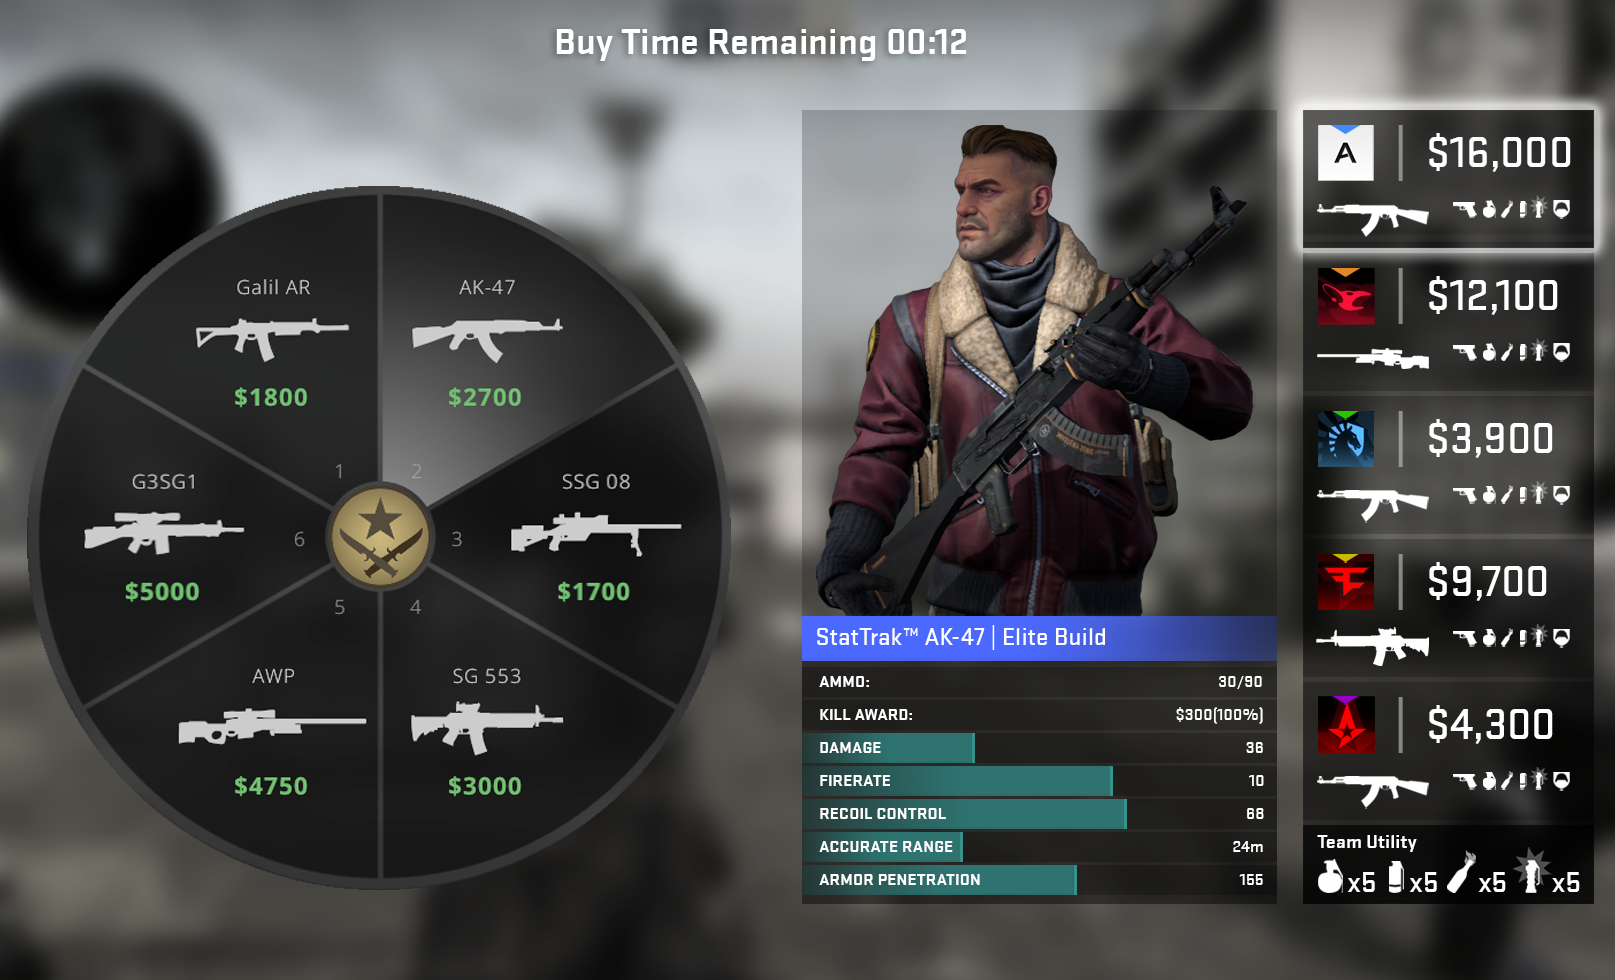
\includegraphics[width=0.9\columnwidth]{game/store.png}
		\caption{\label{fig:store}In-game store example}
	\end{figure}
	
	%\newpage
	
	\subsection{Considerations about the game}
		
		Seeing the gameplay, we thought that this video game was a good candidate for player recognition. 
		Some things that helped us in the educated guess are:
		
		\begin{itemize}
		
			\item The presence of many weapons, divided into six different categories. 
			The personal preference varies for each player and could help in the recognition. 
			\item There are also many possible actions. The number of occurs of every action can help in our task. 
			\item Being an FPS, how each player moves the mouse can be a crucial factor in player recognition.
			\item Most likely also the way one moves can be a major factor in achieving our objective.
		
		\end{itemize} 

%**************************************************************

\section{\label{sec:ml}Machine learning techniques}

	The problem faced is a classification problem. 
	In artificial intelligence, a classification problem is when a machine tries to identify the category of an observation based on previous training. 
	Usually, to achieve this goal, machine learning is a key factor.
	
	\subsection{Model used}
	
		In this chapter, the focus is on presenting the main model used for player recognition.\\
		A powerful class of machine learning algorithms is the one represented by Neural Networks (NN). 
		Neural Networks tries to reproduce biological neural networks, thus are composed of neurons. 
		Artificial Neural Networks' goal is to find patterns in input data, learn from them and generate a corresponding output. 
		Usually, the neurons are organized in ``layers'', which are a set of connected neurons. 
		There are typically three types of layers. 
		These are the input layer (receives data), the hidden layer (finds the patterns), and the output layer (produces results). 
		The connections between the neurons are weighted so that the network can learn only the relevant patterns. 
		The weights are tuned using backpropagation during the training phase.\\
		Figure \ref{fig:nn} shows an example of neural network. 
		
		\begin{figure}[!h] 
			\centering 
			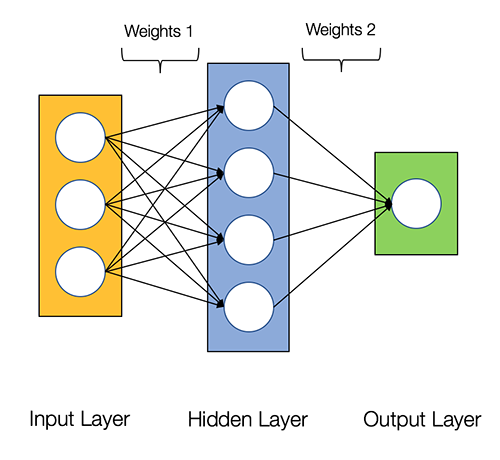
\includegraphics[scale=0.4]{nn/NN.png}
			\caption{\label{fig:nn}Example of neural network}
		\end{figure}
		
		\newpage
		
		A neural network is ``deep'' if there is more than one hidden layer. 
		Deep neural networks are usually used because can understand more complex patterns. 
		A particular deep learning neural network is the Recurrent Neural Network (RNN), which can work with sequences and learn temporal patterns. 
		This peculiarity is achieved with a particular structure of the hidden layer. 
		The information gets stored in the hidden layer and passed to the following one. 
		It can be seen as multiple copies of one neural network, each one passing a message to the following one.\\
		Figure \ref{fig:rnn} shows an RNN, where $A$ is the network, $x_i$ si the input at time $i$ and $h_i$ is the output at time $i$.
		
		\begin{figure}[!h] 
			\centering 
			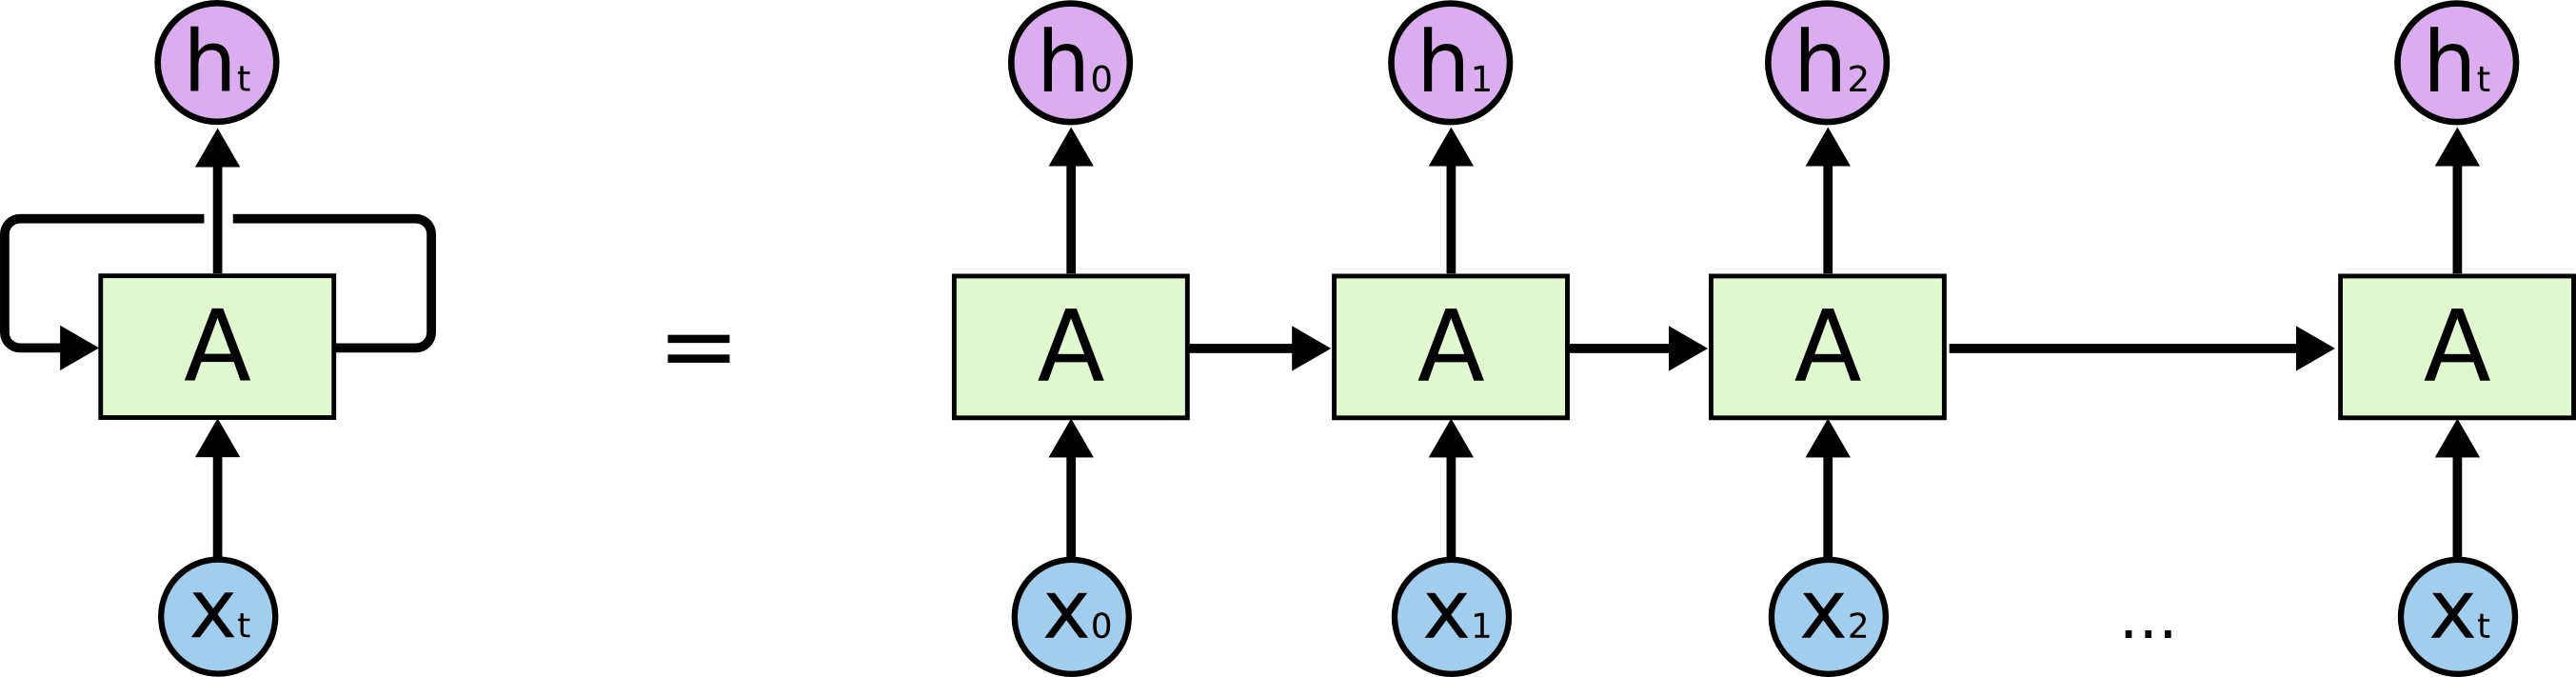
\includegraphics[width=0.9\columnwidth]{nn/RNN.png}
			\caption{\label{fig:rnn}Example of a RNN.}
		\end{figure}
		
		Formally, a Recurrent Neural Network is defined as: \\
		
		\begin{center}
			\begin{equation}
				\begin{aligned}
					$h_t\ =\ \phi (W \ \cdot \ x_t \ + \ U \ \cdot \ h_{t-1})$ \label{for:rnn} \noalign{\vskip1pt}
				\end{aligned}
			\end{equation}
		\end{center}
		
		where W and U are the weight matrix and the transition matrix respectively. 
		$\phi$ is the activation function. 
		The two matrices are used to determine which and how important is the information in the hidden layers. 
		RNN can be very useful, but there are two problems with this kind of neural network. 
		These two problems are known as ``exploding gradient'' and ``vanishing gradients''~\cite{REHMER20201243}. 
		These 2 problems are both resolved using Long Short Term Memory (LSTM)~\cite{10.1162/neco.1997.9.8.1735}.
		This type of neural network is organized in cells (shown in Figure \ref{fig:cell})
		
		\begin{figure}[!h] 
			\centering 
			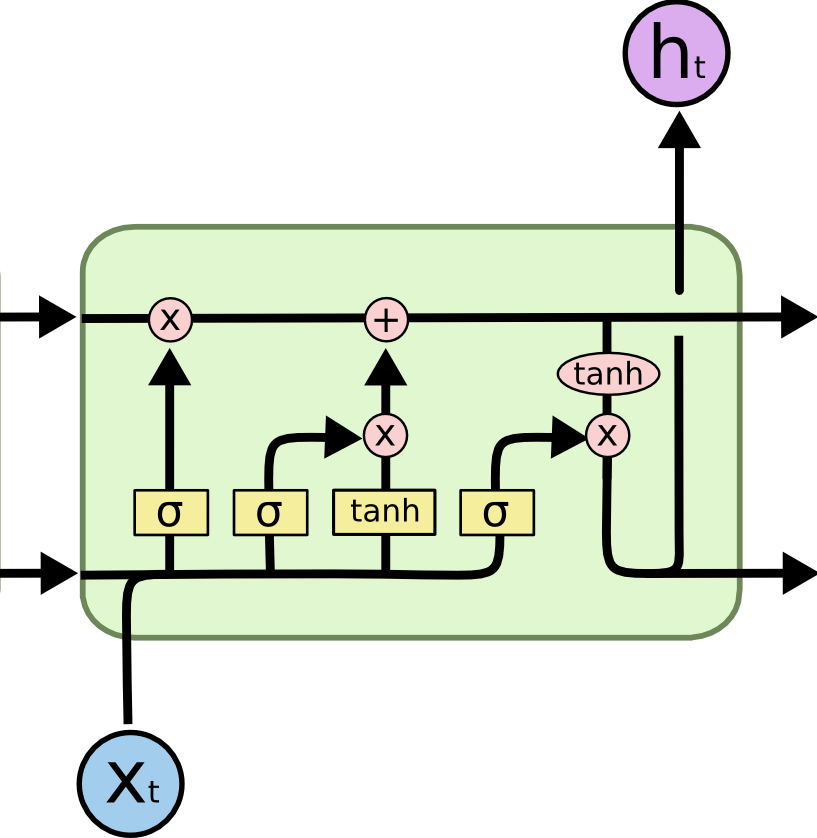
\includegraphics[scale=.35]{nn/LSTM.png}
			\caption{\label{fig:cell}Example of a LSTM cell}
		\end{figure}
		
		The solution to the two mentioned problems is represented by the structure of the cells. 
		There are three structures called gates that control the input and help achieve this goal.
		The gates' name are forget gate, input gate and output gate.
		
		\begin{figure}[!h] 
			\centering 
			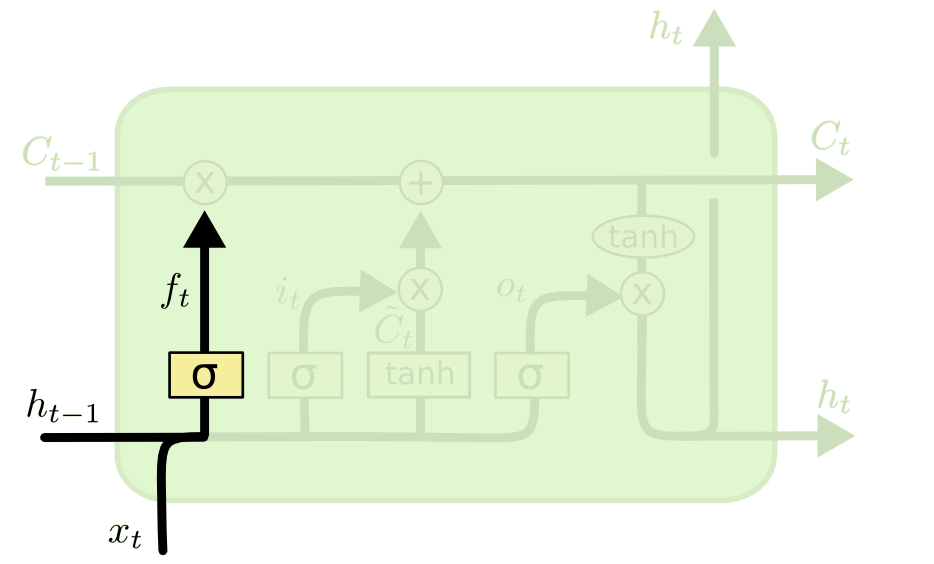
\includegraphics[scale=.7]{nn/LSTM_step1.png}
			\caption{\label{fig:step1}First step of a LSTM neural network}
		\end{figure}
		
		In Figure \ref{fig:step1} is shown how the LSTM uses the forget gate to decide what to forget about the cell state.
		The formula used is:
		\begin{center}
			\begin{equation}
				\begin{aligned}
					$f_t\ =\ \sigma (W_f\ \cdot \ [h_{t-1}, x_t] + b_f)$, \label{for:fg}\noalign{\vskip1pt}
				\end{aligned}
			\end{equation}
		\end{center}
		
		where $h_{t-1}$ is the output of the previous cell, $x_t$ is the input at time $t$, $W$ is the weight matrix, and $b_f$ is the bias vector.
		The output value, scaled between 0 and 1 with a sigmoid function, helps to understand how much to consider from the previous state. 
		
		\begin{figure}[!h] 
			\centering 
			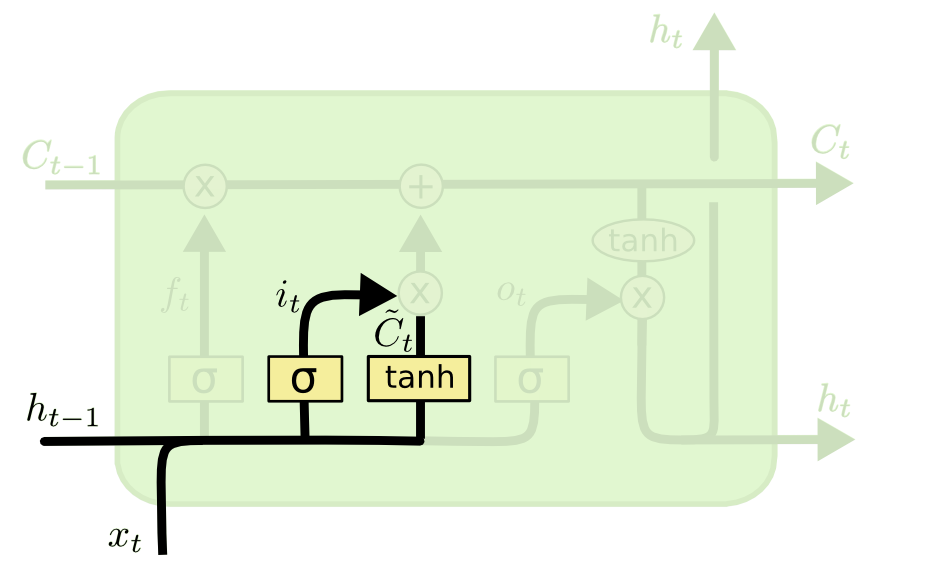
\includegraphics[scale=.7]{nn/LSTM_step2.png}
			\caption{\label{fig:step2}Second step of a LSTM neural network}
		\end{figure}
		
		Figure \ref{fig:step2} shows the second step of the forward propagation of a LSTM cell.
		First, a sigmoid layer (the input gate) decides what to update using the following formula:
		
		\begin{center}
			\begin{equation}
				\begin{aligned}
					$i_t\ =\ \sigma (W_i\ \cdot \ [h_{t-1}, x_t] + b_i)$ \label{for:ig}\noalign{\vskip1pt}
				\end{aligned}
			\end{equation}
		\end{center}
		
		Next, a $\tanh$ layer creates a new vector of candidate values. 
		The candidates values, identified with $\tilde{C_t}$, are computed as:
		
		\begin{center}
			\begin{equation}
				\begin{aligned}
					$\tilde{C_t}\ =\ \tanh (W_C\ \cdot \ [h_{t-1}, x_t] + b_C)$ \label{for:ig2}\noalign{\vskip1pt}
				\end{aligned}
			\end{equation}
		\end{center}
		
		\begin{figure}[!h] 
			\centering
			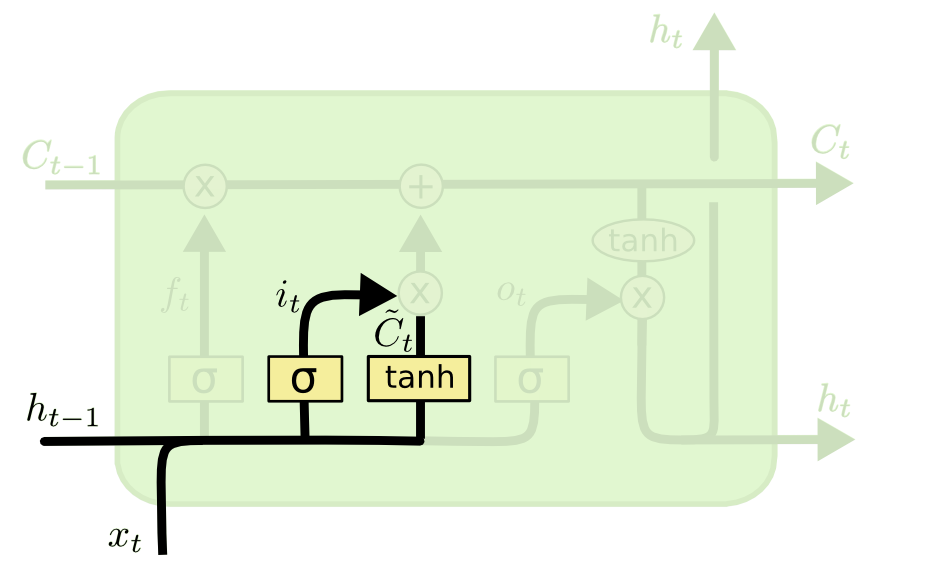
\includegraphics[scale=.7]{nn/LSTM_step2.png}
			\caption{\label{fig:step3}Third step of a LSTM neural network}
		\end{figure}
		
		Figure \ref{fig:step3} shows how the state of the cell changes. 
		First the previous cell state gets multiplied by the output of the forget gate with an element-wise operation.
		Second the values calculated in \ref{for:ig} and \ref{for:ig2} gets multiplied with another element-wise operation and then added to the state cell.
		The formula that can summarize this operation is:
		
		\begin{center}
			\begin{equation}
				\begin{aligned}
					$C_t\ =\ \tanh (f_t\ \cdot \ C_{t-1} + i_t\ \cdot \ \tilde{C_t})$ \label{for:add}\noalign{\vskip1pt}
				\end{aligned}
			\end{equation}
		\end{center}
		
		\begin{figure}[!h] 
			\centering 
			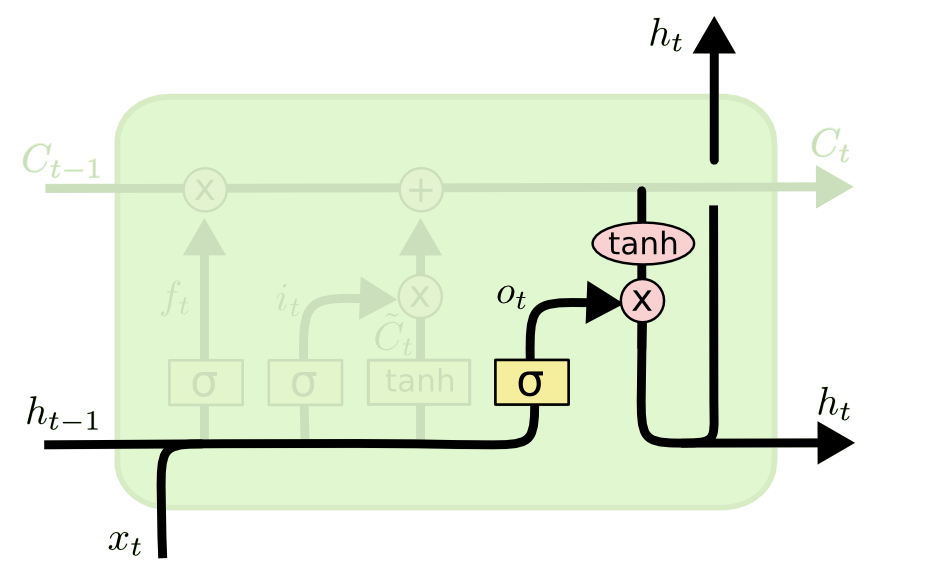
\includegraphics[scale=.7]{nn/LSTM_step4.png}
			\caption{\label{fig:step4}Fourth step of a LSTM neural network}
		\end{figure}
		
		Lastly, figure \ref{fig:step4} shows how the cell decide what to output.
		First, a sigmoid layer decides what to output.
		Then a $\tanh$ layer scales all the values of the cell state between $-1$ and $1$.
		Finally the network performs an element-wise multiplication of the cell state and the output of the sigmoid layer. 
		This process can be summarized with the following formulas:\noalign{\vskip1pt}
		\begin{center}
			\begin{equation}
				\begin{aligned}
					$o_t\ = \ \sigma(W_0 [h_{t-1}, x_t] + b_o)$\\ \noalign{\vskip1pt}
				\end{aligned}
			\end{equation}
		\end{center}
		\begin{center}
			\begin{equation}
				\begin{aligned}
					$h_t\ = \ o_t \ \cdot \ \tanh(C_t)$\noalign{\vskip1pt}
				\end{aligned}
			\end{equation}
		\end{center}
		
	\subsection{Loss function}
	
		During the learning process it is the goal of the model to find the best solution. 
		To find the best solution the model evaluates an ``objective function'' and in this particular task we want to minimize the error of the predictions. 
		In order to achieve this goal the objective function, called ``loss'' function, is directly proportional to how much the predicted results differs from the actual result.\\
		In this classification task, given that every sample can be part of only one class, we chose to use a loss function known as Categorical Crossentropy Loss Function.
		Formally this function is defined as:
		
		\begin{center}
			\begin{equation}
				\begin{aligned}
					$L(y, \hat{y})\ = \ -\displaystyle\sum_{j=0}^M \displaystyle\sum_{i=0}^N (y_{ij} * \log (\hat{y_{ij}})) $\noalign{\vskip1pt}
				\end{aligned}
			\end{equation}
		\end{center}
		
		In this formula, $\hat{y}$ is the predicted value, $i$ is the training sample, $j$ is the output node. $\hat{y_{ij}}$ is the prediction of the sample $i$ belonging to the class $j$ and 
		$y_{ij}$ is the actual value. \\

		The categorical crossentropy loss function compares the distributions of the predictions (the predictions of the output layer, one for each class) with the true distribution, where the 
		probability of the true class is 1 and 0 for every other class. 
		The true classes are simply represented as a one-hot encoded vectors, with only one 1 in the true class and 0 elsewhere, and the closer the model’s outputs are to those vectors, the lower the loss is.
	
	\subsection{Metrics adopted}
	
		In this elaborate, we will use some of the most common metrics to evaluate our models: accuracy and precision.
		In Table \ref{tab:cm} is presented a confusion matrix that will help us to describe the mentioned metrics.
	
		\begin{table}[!h]
			\caption{\label{tab:cm}Confusion matrix}
			\centering
			\begin{tabular}{l|l|c|c|}
				\multicolumn{2}{c}{}&\multicolumn{2}{c}{\textbf{Predicted}}\\
				\cline{3-4}
				\multicolumn{2}{c|}{}&\textbf{Positive}&\textbf{Negative}\\
				\cline{2-4}
				\multirow{\textbf{Actual}}& \textbf{Positive} & True positive & False negative \\
				\cline{2-4}
				& \textbf{Negative} & False positive & True negative\\
				\cline{2-4}
			\end{tabular}
		\end{table}
		
		\paragraph{Accuracy}: Accuracy is defined as:
		
			\begin{center}
				\begin{equation}
					\begin{aligned}
						$Accuracy = \dfrac{TP + TN}{FP + TP + TN + FN}$ \noalign{\vskip1pt}
					\end{aligned}
				\end{equation}
			\end{center}
		
			This metric measures the model's performance considering true positives and true negatives against all the dataset's examples.
			A low value indicates a significant difference between predictions and target values. 
		
		\paragraph{Precision}: Precision is defined as:
		
			\begin{center}
				\begin{equation}
					\begin{aligned}
						$Accuracy = \dfrac{TP}{FP + TP}$ \noalign{\vskip1pt}
					\end{aligned}
				\end{equation}
			\end{center}
		
			This metric measures how many of the predicted true values are truly positive. 
			It helps to determine if the classification error with respect to the true positive is high.